% Created 2018-12-13 ju. 20:01
% Intended LaTeX compiler: pdflatex
\documentclass[xcolor={usenames,svgnames,dvipsnames}]{beamer}
\usepackage[utf8]{inputenc}
\usepackage[T1]{fontenc}
\usepackage{graphicx}
\usepackage{grffile}
\usepackage{longtable}
\usepackage{wrapfig}
\usepackage{rotating}
\usepackage[normalem]{ulem}
\usepackage{amsmath}
\usepackage{textcomp}
\usepackage{amssymb}
\usepackage{capt-of}
\usepackage{hyperref}
\usepackage{color}
\usepackage{listings}
\usepackage{mathpazo}
\usepackage{gensymb}
\usepackage{amsmath}
\usepackage{chemarr}%flechas para reacciones químicas (SFER.tex)
\bibliographystyle{plain}
\AtBeginSubsection[]{\begin{frame}[plain]\tableofcontents[currentsubsection,sectionstyle=show/shaded,subsectionstyle=show/shaded/hide]\end{frame}}
\AtBeginSection[]{\begin{frame}[plain]\tableofcontents[currentsection,hideallsubsections]\end{frame}}
\usepackage[emulate=units]{siunitx}
\sisetup{fraction=nice, decimalsymbol=comma, retain-unity-mantissa = false}
\newunit{\wattpeak}{Wp}
\newunit{\watthour}{Wh}
\newunit{\amperehour}{Ah}
\usepackage{steinmetz}
\hypersetup{colorlinks=true, linkcolor=Blue, urlcolor=Blue}
\renewcommand{\thefootnote}{\fnsymbol{footnote}}
\beamertemplatenavigationsymbolsempty
\setbeamertemplate{footline}[frame number]
\setbeamercolor{alerted text}{fg=blue!50!black} \setbeamerfont{alerted text}{series=\bfseries}
\usetheme[hideothersubsections]{Goettingen}
\usecolortheme{rose}
\usefonttheme{serif}
\author{Oscar Perpiñán Lamigueiro}
\date{\url{http://oscarperpinan.github.io}}
\title{Sistemas Fotovoltaicos Autónomos}
\subtitle{Diseño}
\hypersetup{
 pdfauthor={Oscar Perpiñán Lamigueiro},
 pdftitle={Sistemas Fotovoltaicos Autónomos},
 pdfkeywords={},
 pdfsubject={},
 pdfcreator={Emacs 26.1 (Org mode 9.1.14)}, 
 pdflang={Spanish}}
\begin{document}

\maketitle

\section{Dimensionado del SFA}
\label{sec:org016783f}
\begin{frame}[label={sec:org6a01120}]{Objetivo}
\begin{itemize}
\item El dimensionado de un SFA consiste en \alert{decidir el tamaño del
generador fotovoltaico y acumulador} que serán capaces de
\alert{proporcionar la energía requerida} por una determinada carga a partir
de la \alert{radiación disponible} en la zona.

\item Debido al comportamiento aleatorio tanto de la radiación como del
consumo, la \alert{probabilidad de fallo no es nula}.

\item La solución es un compromiso entre el coste y la fiabilidad del
sistema.
\end{itemize}
\end{frame}


\subsection{Nomenclatura}
\label{sec:org6744e42}
\begin{frame}[label={sec:org717f48e}]{Carga}
\begin{description}
\item[{Consumo:}] \(L\)

\item[{Probabilidad de pérdida de carga:}] relación entre la energía que no
puede suministrar el sistema fotovoltaico y la energía solicitada por
la carga durante todo el período de
funcionamiento.$$LLP=\frac{E_{def}}{L}$$
\end{description}
\end{frame}

\begin{frame}[label={sec:orgb33e172}]{Capacidades normalizadas}
\begin{description}
\item[{Capacidad del generador:}] relación entre los valores medios de la
energía que puede producir el generador y la energía consumida por la
carga.
$$C_{A}=\frac{\eta_{G}\cdot A_{G}\cdot\overline{G_{d}}(\beta,\alpha)}{L}$$

\item[{Capacidad de acumulación:}] relación entre la capacidad útil del acumulador y la energía consumida por la carga.
\end{description}
\[
  C_{s}=\frac{C_{U}}{L}=\frac{C_{B}\cdot PD_{max}}{L}
\]
\end{frame}
\subsection{Objetivo}
\label{sec:org333ca88}
\begin{frame}[label={sec:org402e44f}]{Dimensionado}
\begin{block}{La tarea de dimensionar un sistema fotovoltaico consiste en encontrar la mejor solución de compromiso entre coste y fiabilidad.}
\begin{itemize}
\item Diferentes valores de \((C_{A},\, C_{S})\) pueden conducir al mismo
valor de \(LLP\).

\item Cuanto mayor es el sistema, mayor es la fiabilidad, pero mayor es el
coste.
\end{itemize}
\end{block}
\end{frame}


\subsection{Ejemplos}
\label{sec:org95320f3}
\begin{frame}[label={sec:org36c7216}]{Generador grande, acumulador pequeño}
\begin{block}{Combinación de \(C_{A}\) alta y \(C_{S}\) baja}
\begin{itemize}
\item Ciclos diarios con descargas profundas y frecuentes: perjudicial.

\item Ciclos estacionales cortos: beneficioso (no estratificación).

\item Estratificación compensable con sobrecargas controladas.
\end{itemize}
\end{block}
\end{frame}

\begin{frame}[label={sec:org1ec38af}]{Generador pequeño, acumulador grande}
\begin{block}{Combinación de \(C_{A}\) baja y \(C_{S}\) alta}
\begin{itemize}
\item Ciclos diarios con descargas moderadas: beneficioso

\item Ciclos estaciones largos:  perjudicial (favorece sulfatación y estratificación)

\item Baja frecuencia de sobrecargas, estratificación díficil de compensar.
\end{itemize}
\end{block}
\end{frame}

\begin{frame}[label={sec:org3e7efc3}]{Sistemas Híbridos}
\begin{itemize}
\item Cuando \(LLP\) es muy alta (p.e. radioenlaces) o la demanda es muy
elevada (poblados) el generador y acumulador serán excesivamente
grandes.

\item Es habitual incluir un grupo electrógeno que suministra la energía
deficitaria y permite reducir el tamaño del SFA.

\item \alert{Sinergia}:

\begin{itemize}
\item El grupo electrógeno \alert{reduce el tamaño} del \alert{generador FV} y el
\alert{acumulador} sin reducir fiabilidad.

\item El generador fotovoltaico \alert{reduce horas de funcionamiento del grupo}: gasto en combustible y mantenimiento.
\end{itemize}
\end{itemize}
\end{frame}

\subsection{Métodos de dimensionado}
\label{sec:org8ee3e2b}

\begin{frame}[label={sec:org2b38d42}]{Método del LLP}
\begin{itemize}
\item \alert{Series sintéticas} (\guillemotleft{}simuladas\guillemotright{}) de radiación solar que reproducen el comportamiento estadístico en el lugar.
\item Establece valores de \(C_{A}\) y \(C_{S}\) para un consumo determinado con \alert{curvas de isofiabilidad}.
\end{itemize}
\begin{center}
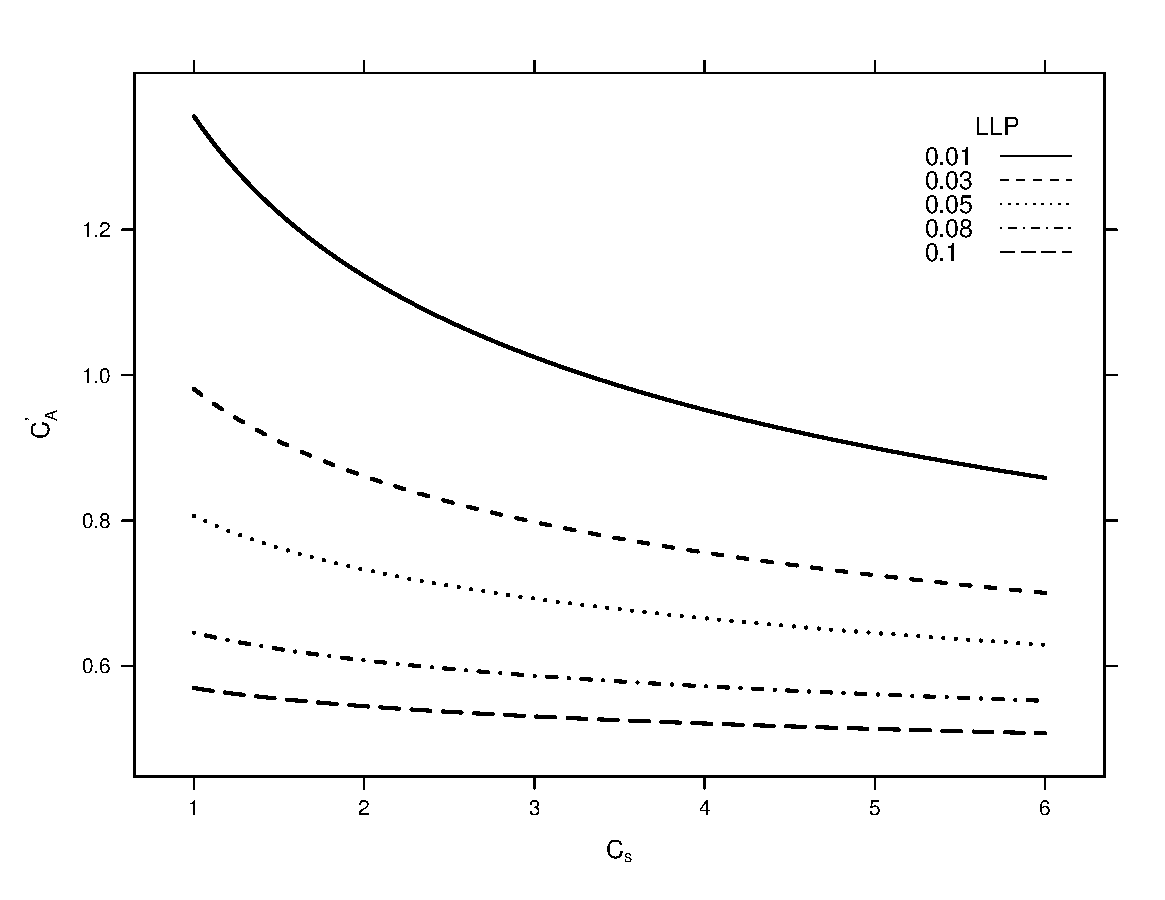
\includegraphics[height=0.65\textheight]{../figs/CurvasLLP.pdf}
\end{center}
\end{frame}

\begin{frame}[label={sec:org1826064}]{Método del mes peor}
\begin{itemize}
\item Determina el tamaño de batería y generador para abastecer el consumo \alert{durante el mes con peor relación entre radiación y consumo}.
\item Si el consumo es constante, el mes peor es aquel de menor radiación.
\item Aplican recomendaciones de expertos según zona geográfica y aplicación (tipología de consumo).
\end{itemize}

\begin{block}{Valores según el UTS for SHS}
\begin{itemize}
\item Electrificación rural:

\begin{itemize}
\item \(C_{A}=1.1\)

\item \(3\leq C_{S}\leq5\)
\end{itemize}

\item Aplicaciones profesionales:

\begin{itemize}
\item \(1.2\leq C_{A}\leq1.3\)

\item \(5\leq C_{S}\leq8\)
\end{itemize}
\end{itemize}
\end{block}
\end{frame}

\subsection{Configuración de generador y batería}
\label{sec:orgbc45554}
\begin{frame}[label={sec:orgb8d8fe1}]{Configuración de generador y batería}
\begin{itemize}
\item Una vez elegidos los valores de \(C_{A}\) y \(C_{S}\), se deben
configurar el generador y batería de acuerdo a las tensiones de
trabajo.

\item En general, la batería impone la tensión de trabajo (no hay buscador
de MPP). Supondremos \(V_{mpp} \simeq V_{b}\)

\item Carga en Ah
\end{itemize}
\[
\boxed{Q_L = L / V_b}
\]
\end{frame}

\begin{frame}[label={sec:org037c78a}]{Batería}
\begin{itemize}
\item Capacidad en Ah (es recomendable no usar baterías en paralelo)
\end{itemize}
\[
C_{s}=\frac{C_{U}}{L}=\frac{C_{B}\cdot PD_{max}}{L} \rightarrow \boxed{Q_B = \frac{C_S \cdot Q_L}{PD_{max}}}
\]

\begin{itemize}
\item Hay que elegir el número de vasos en serie adecuados a \(V_b\)
\end{itemize}
\end{frame}


\begin{frame}[label={sec:org5d8281f}]{Generador}
\begin{itemize}
\item Capacidad del generador
\end{itemize}
\[
C_{A} = \frac{\eta_{G}\cdot A_{G}\cdot\overline{G_{d}}(\beta,\alpha)}{Q_L \cdot V_b}
\]

\begin{itemize}
\item Potencia del generador (suponiendo \(V_{mpp} \simeq V_{b}\))
\end{itemize}
\[
I_{g}^{*}\cdot V_{b} = \eta_{G}\cdot A_{G}\cdot G^*
\]

\begin{itemize}
\item Corriente de funcionamiento (determina número de ramas):
\end{itemize}
\[
\boxed{I_{g}^{*} =  \frac{C_{A}\cdot Q_{L}\cdot G^*}{\overline{G_{d}}(\beta,\alpha)}}
\]

\begin{itemize}
\item Hay que elegir el número de módulos en serie adecuados a \(V_b\)
\end{itemize}
\end{frame}

\begin{frame}[label={sec:org01281ad}]{Inclinación del generador}
\begin{itemize}
\item Para instalaciones con \alert{consumos constantes o similares a lo largo del año}, se busca maximizar la radiación en los meses de menor insolación $$\beta=|\phi|+10^{\circ}$$

\item Para instalaciones con \alert{consumo menor en meses de baja radiación} se busca maximizar radiación en equinoccios.$$\beta=|\phi|$$

\item Para instalaciones con \alert{uso predominante en verano} (hemisferio Norte) conviene emplear un ángulo inferior a la latitud. $$\beta=|\phi|-10^{\circ}$$

\item En general, la inclinación \alert{debe superar} los \(15^{\circ}\).
\end{itemize}
\end{frame}

\section{Consumo}
\label{sec:orge584165}

\subsection{Estimación del consumo}
\label{sec:org14faebf}
\begin{frame}[label={sec:orgb770eec}]{Cálculo del consumo}
\begin{itemize}
\item Energía total requerida por las cargas
\end{itemize}
$$L_{T}=\frac{L_{dc}}{\eta_{r}}+\frac{L_{ac}}{\eta_{inv}}$$

\begin{itemize}
\item Energía producida por el generador
\end{itemize}
$$L=\frac{L_{T}}{\eta_{bat}\cdot\eta_{c}}$$

Como valores orientativos pueden utilizarse

\(\eta_{inv}=0.9\), \(\eta_{r}=0.95\), \(\eta_{bat}=0.85\) y \(\eta_{c}=0.98\).
\end{frame}

\begin{frame}[label={sec:org176a95a}]{Distribución del consumo}
\begin{center}
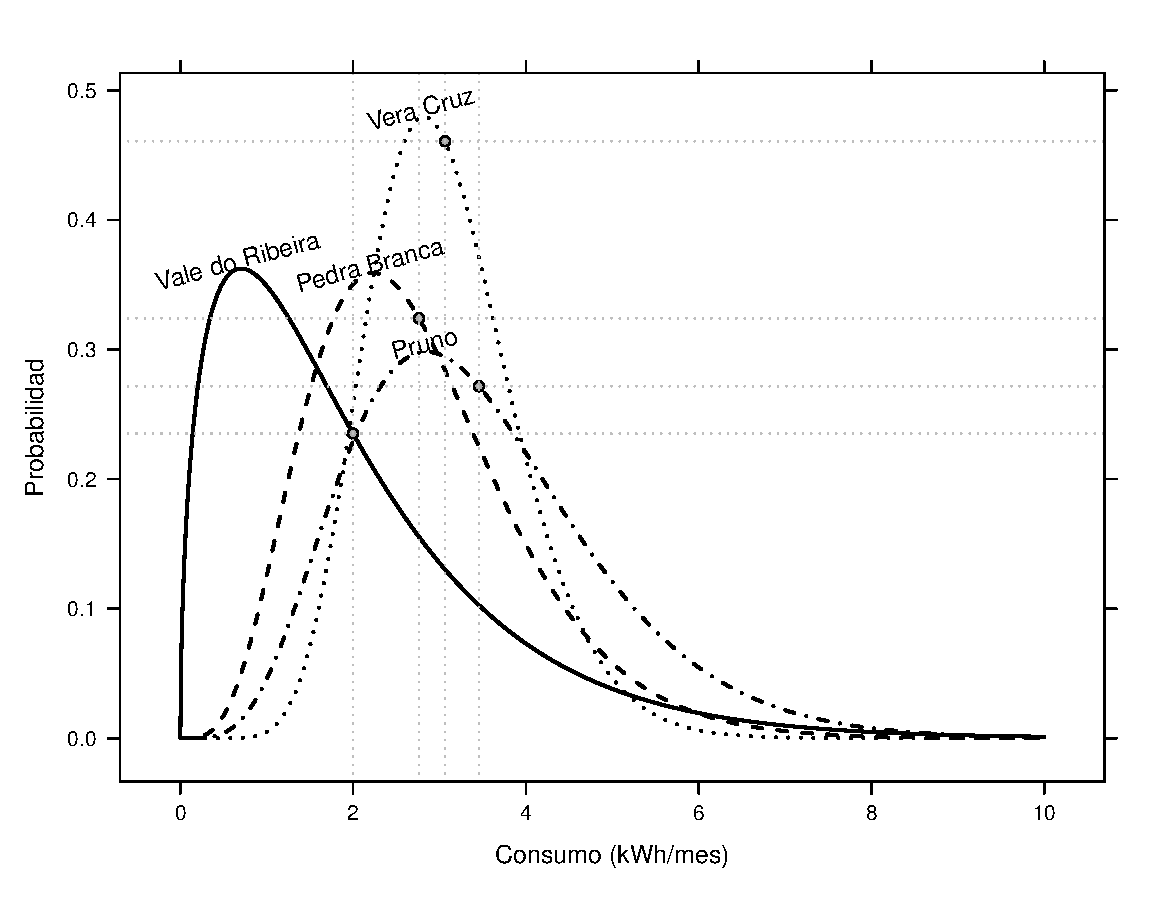
\includegraphics[width=.9\linewidth]{../figs/ConsumoGamma.pdf}
\end{center}

\begin{quote}
'[\ldots{}] mucha gente consume poco y poca gente consume mucho'
\end{quote}
\end{frame}

\begin{frame}[label={sec:org0c0eb92}]{Relación entre el consumo y la fiabilidad}
\begin{itemize}
\item La variación en el consumo se amplifica en la variación de la LLP.
\item \alert{Diseño robusto}: funcionamiento en amplio abanico de condiciones (ambientales y humanas).
\end{itemize}
\begin{center}
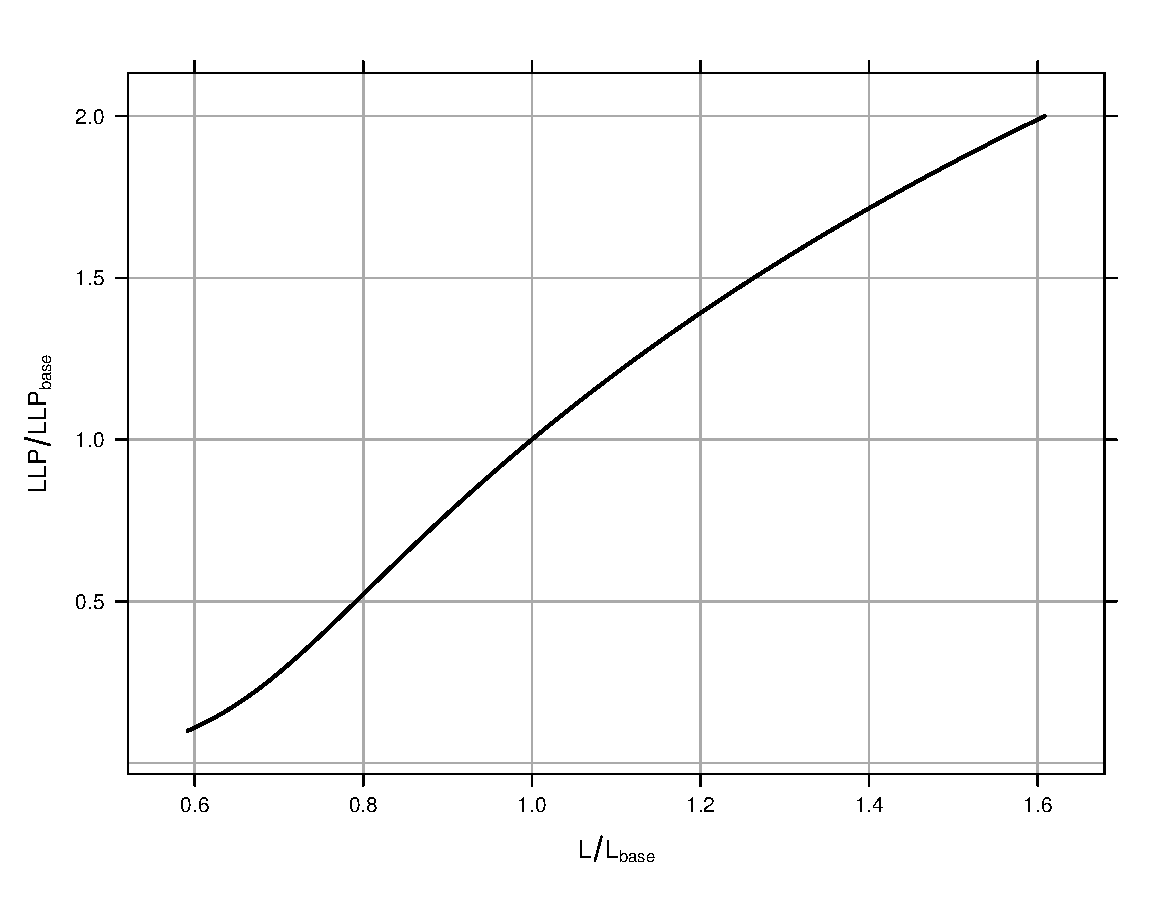
\includegraphics[height=0.7\textheight]{../figs/ConsumoLLP.pdf}
\end{center}
\end{frame}

\subsection{Escenarios de Consumo}
\label{sec:orgb91c376}
\begin{frame}[label={sec:orgf8c9aa5}]{SHS 1}
\begin{block}{120 Wh/dia}
\begin{itemize}
\item Iluminación

\item Radio

\item TV b/n,

\item Sin frigorífico
\end{itemize}
\end{block}

\begin{block}{Valores recomendados}
$$\begin{aligned}
C_{A} & = & 1.1\\
3\leq & C_{s} & \leq5
\end{aligned}$$
\end{block}
\end{frame}

\begin{frame}[label={sec:orgde115a0}]{SHS 2}
\begin{block}{250 Wh/dia}
\begin{itemize}
\item Iluminación

\item Radio

\item TV color

\item Sin frigorífico
\end{itemize}
\end{block}

\begin{block}{Valores recomendados}
$$\begin{aligned}
C_{A} & = & 1.1\\
3\leq & C_{s} & \leq5
\end{aligned}$$
\end{block}
\end{frame}

\begin{frame}[label={sec:orge3aed69}]{SHS 3}
\begin{block}{1000 Wh/dia}
\begin{itemize}
\item Iluminación

\item radio

\item TV color

\item Con frigorífico eficiente
\end{itemize}
\end{block}

\begin{block}{Valores recomendados}
$$\begin{aligned}
C_{A} & = & 1.1\\
C_{S} & = & 5
\end{aligned}$$
\end{block}
\end{frame}

\begin{frame}[label={sec:orgfe3c53f}]{Centrales}
\begin{block}{}
\begin{itemize}
\item Todo AC

\item 500 Wh/dia por vivienda.
\end{itemize}
\end{block}

\begin{block}{Valores recomendados}
$$\begin{aligned}
C_{A} & = & 1.1\\
C_{S} & = & 5\end{aligned}$$
\end{block}
\end{frame}
\end{document}